\begin{savequote}[75mm] 
Quality is never an accident; it is always the result of intelligent effort. 
\qauthor{John Ruskin.} 
\end{savequote}


\chapter{UT test beam analysis - a measurement of the charge sharing
in planar silicon sensors}
\label{chapter:testbeam}

This chapter is dedicated to describes the testbeam studies performed on prototypes of silicon microstrip sensors that will build the Upstream Tracker.  The chapter starts by presenting the general idea of the testbeam experiments, followed by a section on an experimental setup. The final section describes the study on charge sharing phenomena and the proposed correction. 

\section{Experimental setup}

\subsection{The beam}
The tests were performed in CERN SPS North Area, see figure \ref{fig:LHC}. The beam consisted of secondary particles produced by the interaction of high intensity of 450 GeV/c primary proton beam with a fixed target made of beryllium and lead. The beam had average energy of $180 GeV$.  
The beam typically produced four spills/minute. The spill lasted about 4 seconds, and it was intermittent by 40 seconds window with no beam. For most of the data taking, the beam size was collimated down to about 0.5 cm in diameter.

\subsection{Timepix3 telescope}
The essential tool that allows making many silicon sensor performance studies is the TimePix3 telescope, presented in figure \ref{fig:telescope}. 


\begin{figure}[!h]
\centering
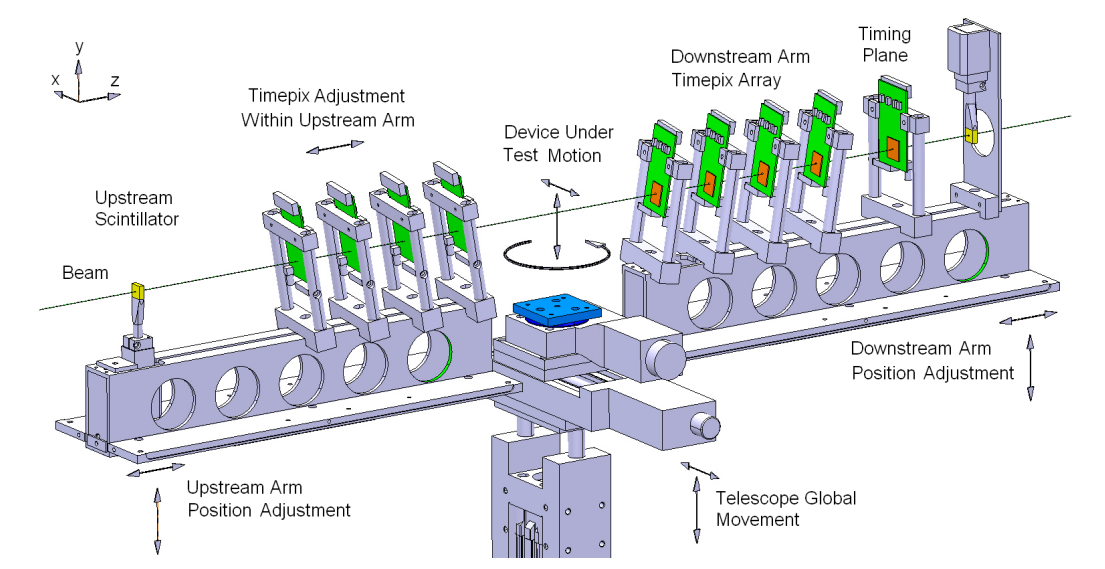
\includegraphics{figures/telescope.png}
\caption{Layout of the Timepix Telescope mechanics, pixel planes and scintillators with respect to the beam axis. Figure taken from \cite{telescope}}
\label{fig:telescope}
\end{figure}


This device consists of 8 plates of 300 $\mu m$ thick p-on-n sensors bump bonded to the Timepix3 ASIC, divided equally between two arms. The position of each plate along the z-axis is adjustable, typically the distance between each plate is set to be 31 mm, and plates are rotated to an angle of 9 deg in both x and y-axis to improve position reconstruction. There is a 200 mm gap between two telescope arms, which is used to place Device Under Test (DUT), see photography \ref{fig:telescope_photo} taken during one of the testbeam companies. The DUT is housed inside a metal box designed to fit into the gap and provides an airtight dry environment cooled via a Peltier device. 
The DUT was installed on a motion stage allowing angular rotations, and x and y translations. 

To allow the DUT acquisition to trigger two scintillators are placed upstream and downstream of the telescope. The telescope acquisition system does not require any trigger signal since it works in a so-called data-driven read-out mode in which the data package of each pixel hit is sent immediately after Time-over-Threshold (ToT) conversion. To synchronize DUT clusters with associated Telescope tracks, the information about the trigger timestamp is added to the data recorded by the telescope. To leverage the tracking information, the algorithm to match the UT clusters with corresponding telescope track was implemented. 


\begin{figure}[!h]
\centering
\hspace*{-1cm}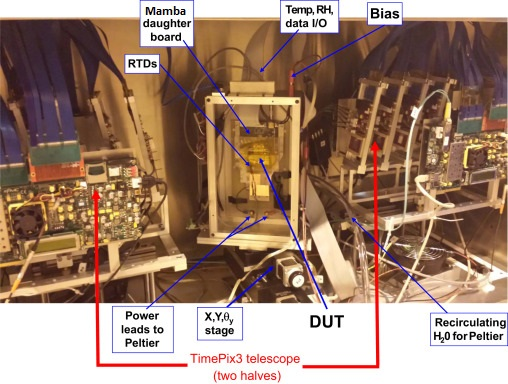
\includegraphics{figures/telescope_photo.jpg}
\caption{The photo of the Timepix Telescope and the DUT inside the box. }
\label{fig:telescope_photo}
\end{figure}

\subsubsection{TimePix3 Telescope Tracking}

To find the position where the particle interacts with the DUT sensor, the particle trajectory needs to be reconstructed using the information provided by all Telescope plates. This procedure starts by finding clusters. The cluster is a collection of neighboring pixels in which the measured signal exceeds a certain threshold, and such a measurement is called a hit. The hit is created when a charged particle traverses through the sensor.  To add the hit to the cluster, its timestamp must lie within the 100 nanosecond window surrounding the timestamp of the seed hit. The timestamp of the cluster is a minimum of the timestamps associated with each of the hits belonging to the cluster. The cluster charge is a sum of charges of the constituent hits. 
The x and y positions of the cluster are calculated using the center of gravity method: 

\begin{equation}
    \{x,y\}_{cluster} = \frac{\sum_{i = 0}^{n} \{x,y\}_{i} S_{i}}{\sum_{i = 0}^{n} S_{i}} 
\end{equation}
where $\{x,y\}_{i} $ is the $x$ or $y$  coordinates of $i$th pixel and $S_i$ its signal. 

The clusters are then used as input for the tracking algorithm, which is based on the timing information of the clusters.  The tracking algorithm starts by taking a cluster form the first plane and then looks for the matching cluster on the second plane. The hits are considered matched when the time difference is within ten nanoseconds. These two clusters constitute a track seed which is then extrapolated to the next plane, excluding the device under test, looking for a cluster within a cone with an opening angle of 0.01 radians and the ten nanoseconds time window. The procedure ends when all planes have been considered. Figure \ref{fig:telescope_tracks} shows four examples of Timepix3 tracks. 



\begin{figure}
\centering
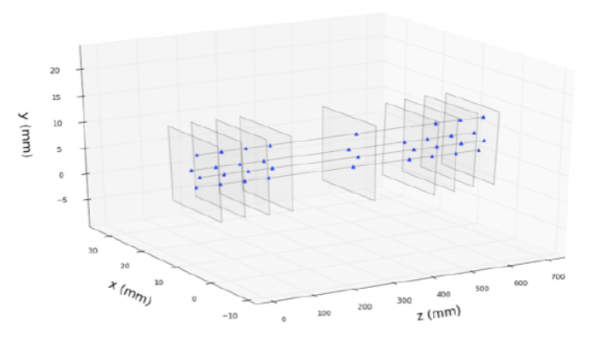
\includegraphics[scale=0.9]{figures/telescope_tracks.png}
\caption{Four exemplary tracks reconstructed in the Timepix3 telescope. Figure taken from \cite{Sophie}.}
\label{fig:telescope_tracks}
\end{figure}


\subsection{Read-out electronic}
During all of the testbeam experiments conducted from 2015 till 2017, the SALT ASIC was not ready. Therefore, the sensor was read-out by the Beetle chip, which is the ASIC used as a front-end chip in Velo and TT during Run 1 and Run 2. The Beetle chip can read-out the signals from 128 channels and returns semi-Gaussian analog pules. The detailed description of the Beetle chip data processing can be found \cite{Beetle}. In contrary to the SALT ASIC, the Beetle chip has no digital signal processing module. Thus, data have to digitalized and processed by the external components.  
The analog data read-out by the Beetle chip was digitalized by the Mamba board designed by INFN in Milan and produced by Nuclear Instrument \cite{NuclearInstruments}.   
The processing of the digitalized data was done by the software described in chapter \ref{chapter:tbut}. 

\section{Testbeam studies and the results}
In the course of the last five years, the LHCb UT Upgrade team has organized a number of testbeam campaigns to test new prototyped sensors. Figure \ref{fig:DUT} presents the photography of a sensor that was used during the testbeam with equipment which allowed to cool
them and collect the data. 

\begin{figure}
\centering
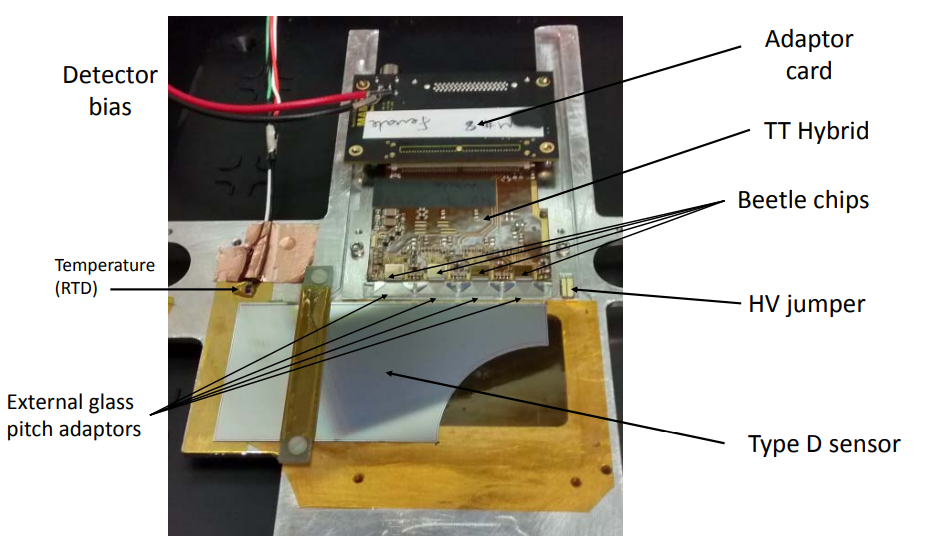
\includegraphics{figures/Sensor_photo.PNG}
\caption{Photo of the D-type sensor that were studied during 2015 testbeam.}
\label{fig:DUT}
\end{figure}



During this testbeams, the following tests were conducted: 

\begin{itemize}
\item Landau distribution as a function of bias voltage. This test scenario was executed to measure the influence of radiation fluence on a Signal to Noise ratio (S/N).  For each sensor, the data was collected at bias voltages ranging from well below the full depletion region (about 50V) to the region well above it (usually 500V).
\item  Cluster size vs. bias voltage and angle of incidence. This study was performed to understand the effect of charge sharing in high irradiated sensors. 
\item Cluster charge vs. cluster size and interstrip position. In this section, the team investigates the dependence of the collected charge on the cluster size. With no radiation effects, one would expect that the collected charge to be independent of the cluster size. However, radiation effects can lead to a difference which was investigated. 
\item Cluster size and resolution vs. angle.  Studies of the detector performance were also carried out at angles ranging from normal incidence to 30 o (with respect to the normal to the sensor). 
\item Charge collection near the quarter-circle region. One type of sensor that will constitute the UT sensor has a quarter-circle region where there are no strips. This study aimed to investigate whether there is any drop in charge collected as a cluster approaches the quarter-circle radially. 
\end{itemize}

The results of this studies lead to the following publications \cite{tb1} \cite{tb2} \cite{tb3}. To get a broader picture of the UT testbeam studies, one can also refer to these PhD thesis \cite{Federica} and \cite{Kelsey}.


\section{Cross-talk correction}
\label{sec:cross_talk}
One of the effects that may influence sensor performance measurements is an asymmetric cross-talk between $N$-th and $(N+1)$-th channel. This effect can be measure by studying the asymmetry between $(N-1)$-th and $(N+1)$th channel, where $N$-th channel is a cluster seed strip position. The effect was studied separately for odd and even channels since it was observed, that this cross-talk effect is stronger for even channels, see figure \ref{fig:charge asymmetry profile}.  


\begin{figure}[htb]
\centering
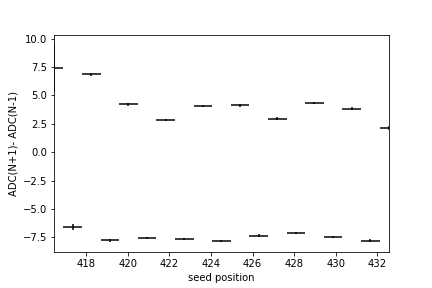
\includegraphics[scale=0.5]{figures/eta/profile_0deg.png}
\caption{The charge collection difference ($ADC(N+1) - ADC(N-1)$) as a function of the strip position. The statistical uncertainty, which were calculated for each bin independently, are shown as one standard deviation. }
\label{fig:charge asymmetry profile}
\end{figure}

To get a better understanding of the signal cross-talk effect on a collected data, the difference between $ADC(N-1)$ and $ADC(N+1)$ as a function of a cluster charge was studied. Figure \ref{fig:difference_odd_even} shows that this difference is strongly dependent on a cluster charge. Thus any proposed correction should take this fact into consideration.  The idea to correct this effect is to create a two-dimensional map with a strip position and cluster charge as indexes and a correction as a value. The correction can be modeled using Gaussian distribution since it was empirically discovered that the charge difference is normally distributed.
Therefore the correction algorithm splits the cluster data into bins according to strip position $N$ and the cluster charge, then for each of the bin, the correction is calculated by fitting Gaussian distribution to the charge difference  $ADC(N-1)$ and $ADC(N+1)$. 
Figure \ref{fig:correction} present this correction calculation procedure for cluster seed charge between 300 and 400 ADC, and figure \ref{fig:correction_map} present the entire 2D correction map. 

\begin{figure}[htb]
\begin{center}
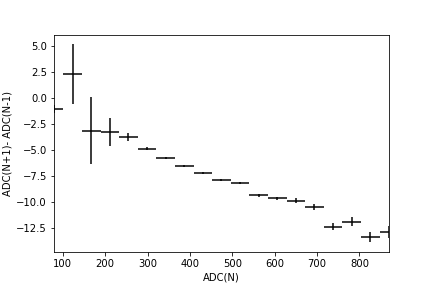
\includegraphics[width=0.49\textwidth]{figures/eta/difference_vs_charge_even.png} 
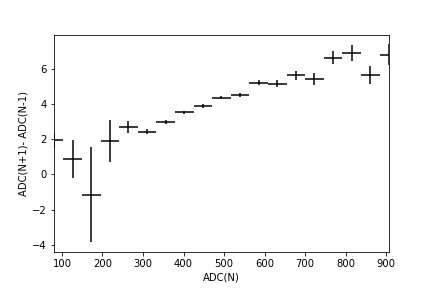
\includegraphics[width=0.49\textwidth]{figures/eta/difference_vs_charge_odd.png}
\caption{The charge collection difference ($ADC(N+1) - ADC(N-1)$) as a function of the cluster charge collected in channel $N$. The left plot shows the difference value for even strips while right plot for even ones }
\label{fig:difference_odd_even}
 \end{center}
 \end{figure}



\begin{figure}[htb]
\begin{center}
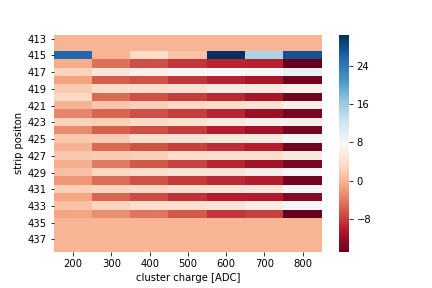
\includegraphics[scale=0.7]{figures/eta/correction_2d.png} 
\caption{Cross-talk correction map. The color indicates value of the correction obtained from the Gaussian fit to the charge difference ($ADC(N+1) - ADC(N-1)$).}
\label{fig:correction_map}
 \end{center}
 \end{figure}



\begin{figure}[h]
\begin{center}
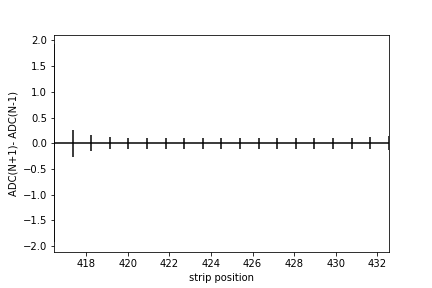
\includegraphics[width = 0.49\textwidth]{figures/eta/difference_ac.png} 
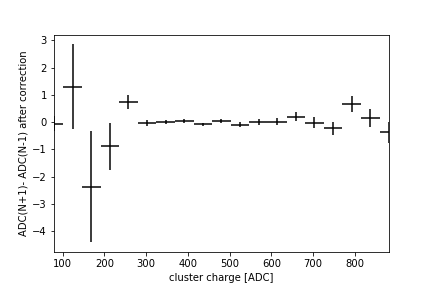
\includegraphics[width = 0.49\textwidth]{figures/eta/difference_vs_charge_ac.png}
\caption{The charge difference ($ADC(N+1) - ADC(N-1)$) after 2D correction as a function of the cluster charge collected in channel $N$ (left) and cluster charge (right). }
\label{fig:after_correction}
 \end{center}
 \end{figure}


\begin{figure}
\centering
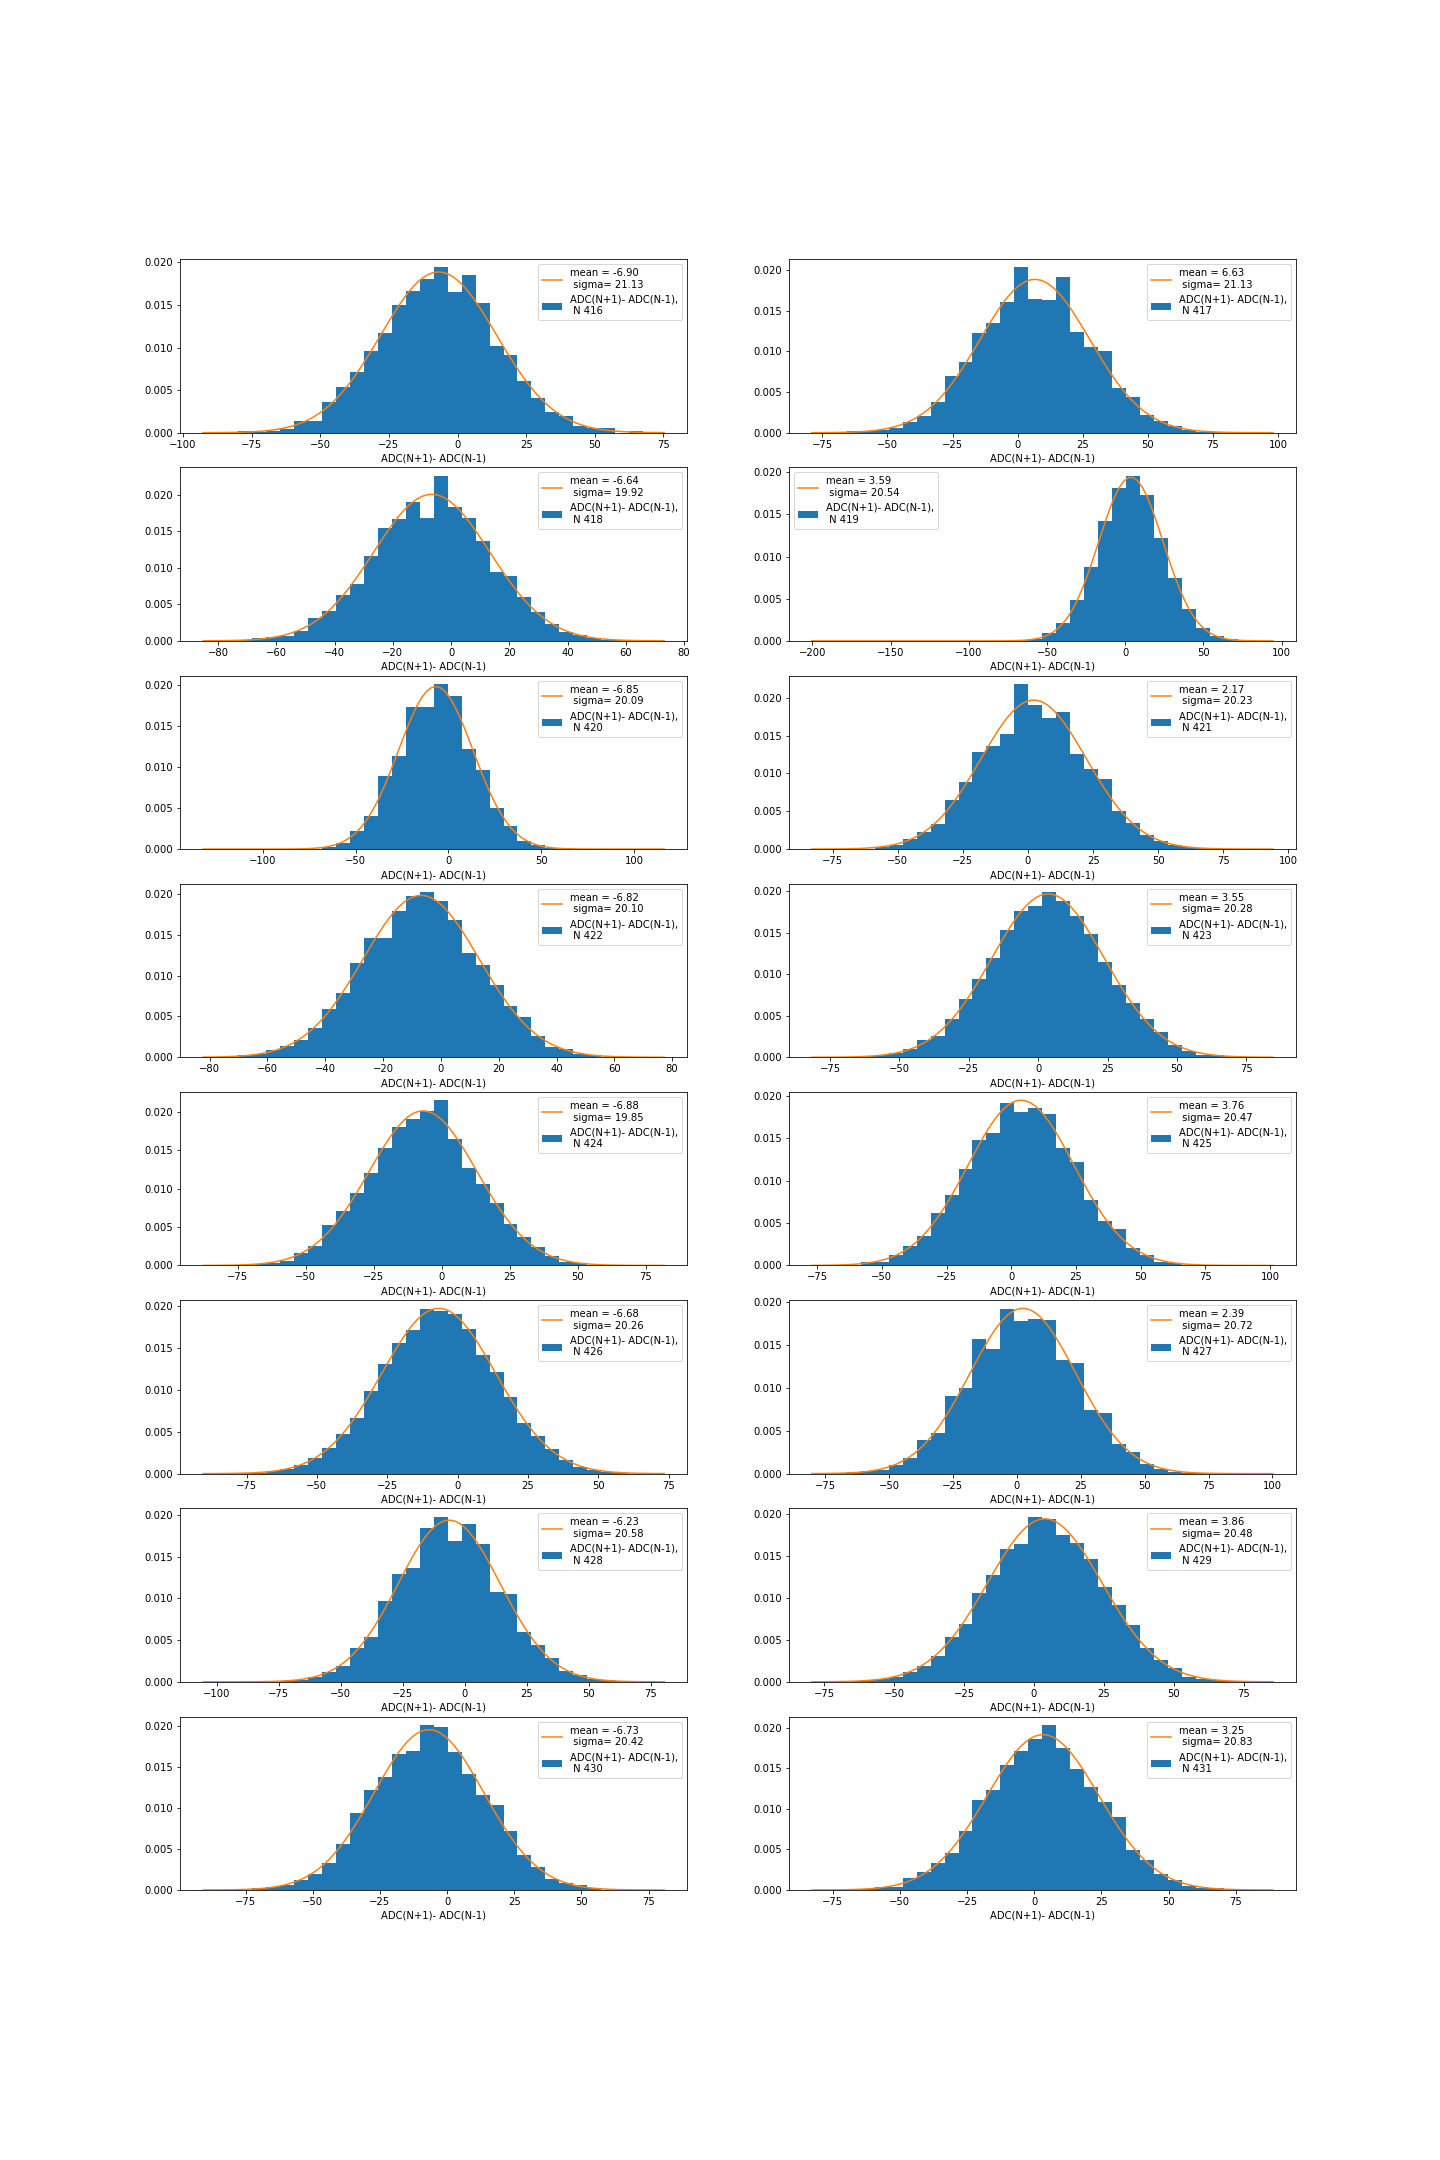
\includegraphics[width=\textwidth]{figures/eta/correction.png}
\caption{The cross-talk correction procedure visualization. Left plots shows charge difference for odd channels while the right plots presents same distribution for even channels. The data was fitted with a Gaussian distribution. } 
\label{fig:correction}
\end{figure}


After application of this correction the cross-talk is not detectable anymore, since the difference is smaller than 1 ADC, see figure \ref{fig:after_correction}. 
All DUTs have similar odd–even cross-talk corrections. The even/odd cross-talk correction was similar for all of the DUTs, but not identical. Therefore, each sensor had a unique cross-talk correction to remove this bias.



\section{Charge sharing}
Charge sharing is manifested when a particle deposits charge between two strips.  In this case, the charge can flow to both the left and right strips, see figure \ref{fig:eta}. The theoretical explanation of this effect can be seen as a transverse diffusion of the holes (or electrons) during the drift towards the strip implant \cite{semiconductors_det_sys}. 
 

\begin{figure}[htb]
\centering
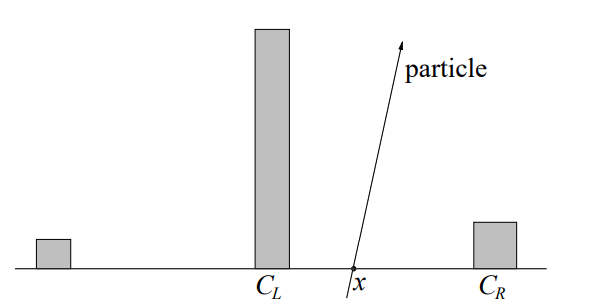
\includegraphics[scale=0.8]{figures/eta/eta.PNG}
\caption{Cartoon of the charge deposited by a particle passing through the silicon. The charge, $C_{\{L, R\}}$, is deposited on the strips left and right of the particle’s impact point x. On the far-left strip some charge is measured as well due to capacitive coupling. Figure adapted from \cite{eta_note} } 
\label{fig:eta}
\end{figure}

This phenomenon can be quantified via parameter $\eta$, proposed in \cite{eta}, given by:
\begin{equation}
    \eta = \frac{Q_{left}}{Q_{left}+Q_{right}}
\end{equation}

The effect of charge sharing were analyzed with respect to the cluster interstrip position and the rotation angle. Each distribution was fitted with an error function model given by:

\begin{equation}
\label{eq:eta_model}
f(x;\sigma) = a \left(1 - erf(\frac{x-\mu}{\sqrt{2}\sigma})\right) + b
\end{equation}

where $a$, $b$ are constants,  $\mu$ is a mean interstrip position, $\sigma$ is a width and $erf$ is the Gauss error function given by:
\begin{equation}
erf(x) = \frac{2}{\pi} \int^{0}_{x} e^{-t^2} dt
\end{equation}

This charge sharing non-linear model can be interpreted as a smeared step function in which the width of the charge sharing ($ \sigma $) equals the width of the Gaussian smearing.   The full derivation of this formula can be find \cite{eta_note}. 

The purpose of this analysis was to measure the dependence of charge sharing $ \eta $ versus the angle of particle incidence.  Different incidence angles were obtained by rotating the stage where the DUT box was mounted around the $y$ axis. 

The data that were used within this analysis comes from May 2016 testbeam.  This section presented studies related to one selected unirradiated mini sensor produced by Hamamatsu Photonics \cite{Hamamatsu}. The sensor is $p^{+}-on-n$ and has a thickness of $320 \mu m$ and a pitch of $190 \mu m$. The clusters that were considered during the presented have to lie in the beam region, be matched with a telescope tracks.  Moreover, the reconstruction quality of those matched tracks should also be satisfactory ($\chi^{2}\/ndf<10$).
Finally the cross-talk correction described in section \ref{sec:cross_talk} was applied.

Figure \ref{fig:eta_distribution} present the $\eta$ distributions integrated overall connected and not masked channels of the mini sensor. Each subfigure is dedicated to present the  $\eta$ for a different particle incidence angle. 
The charge sharing seems to be symmetric, thus no further correction was recommended. 

To get a better understanding of the charge sharing, its dependence versus the cluster interstrip position on the rotation around the $y$-axis is shown in figure \ref{fig:eta_distribution_2d}. Figure \ref{fig:eta_fit} presents same distribution but with mode \ref{eq:eta_model} fitted to the data. One can find that the effect of clockwise and anticlockwise rotations around the $y$-axis is the same.  The $\sigma$ as a function
of the particle incident angle have a minimum at zero degrees and to is symmetrically distributed around the minimum. The effect of a rotation around the $y$-axis is to increase the charge sharing between neighbouring strips, which can be quantified using the value of $\sigma$ obtained from the fit. 


\begin{figure}[bph]
\begin{center}
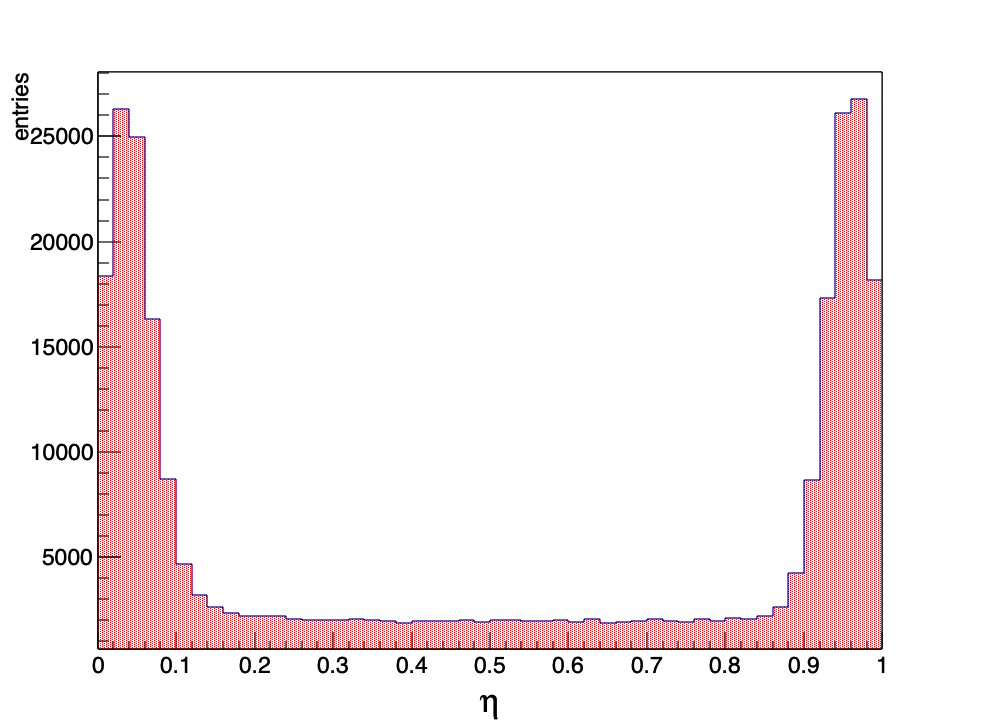
\includegraphics[width = 0.49\textwidth]{figures/eta/eta_1d_10.png} 
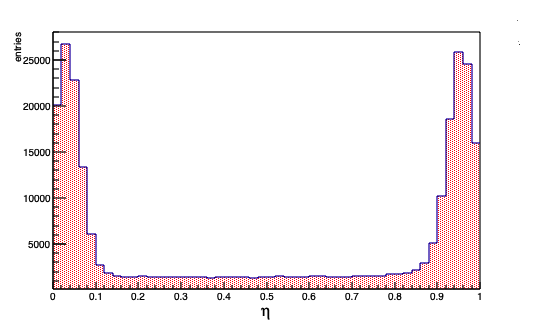
\includegraphics[width = 0.49\textwidth]{figures/eta/eta_1d_neg10.png}
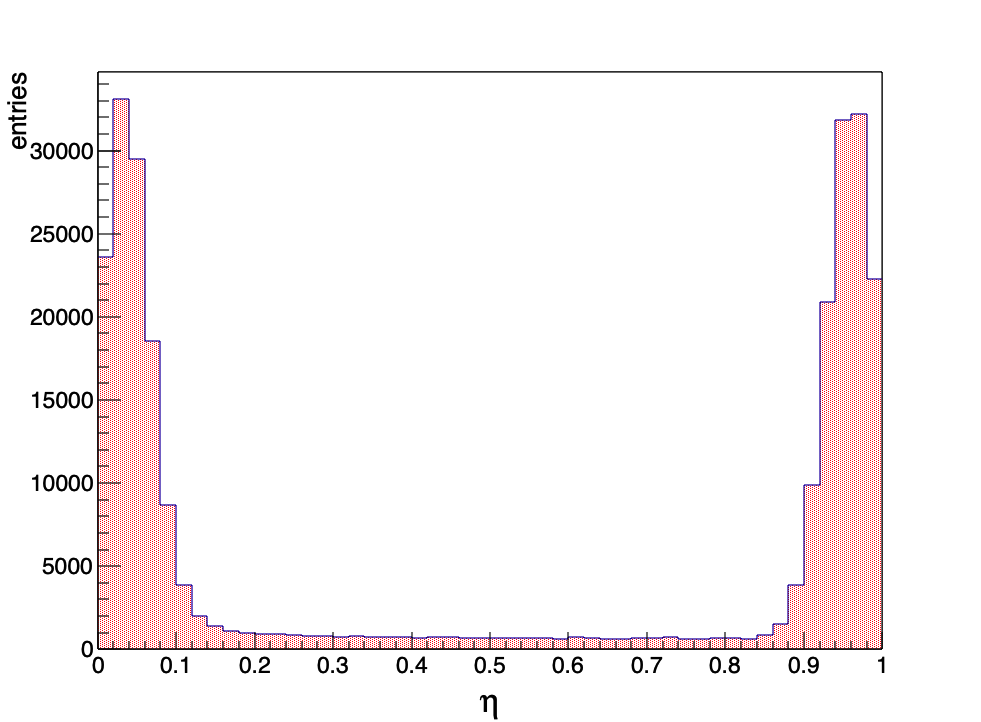
\includegraphics[width = 0.49\textwidth]{figures/eta/eta_1d_2.png} 
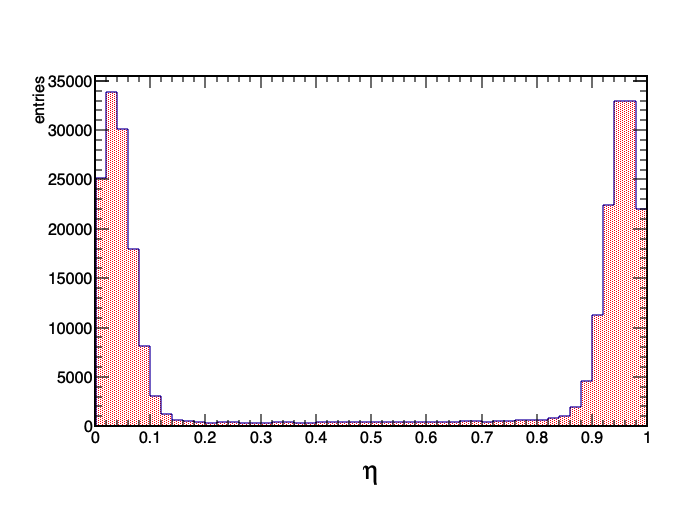
\includegraphics[width = 0.49\textwidth]{figures/eta/eta_1d_neg2.png} 
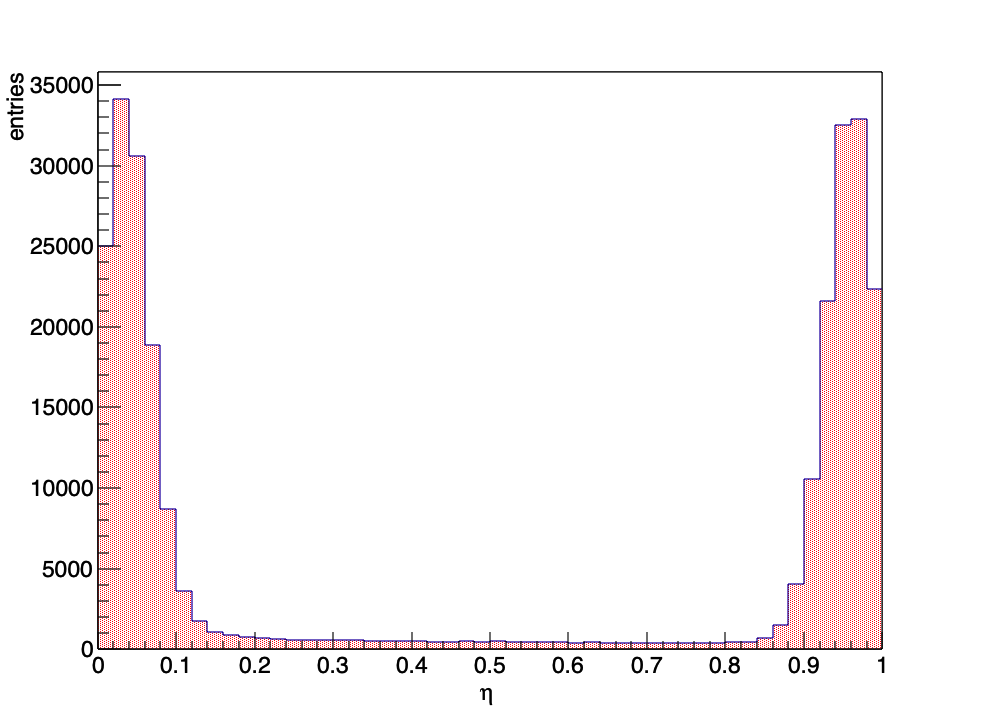
\includegraphics[width = 0.49\textwidth]{figures/eta/eta_1d_0.png} 

\caption{Distribution of a charge sharing $\eta$ obtained for particles incident at a different angle. Upper row $10^{\circ}$ and $-10^{\circ}$, middle row $-2^{\circ}$ and $2^{\circ}$, bottom row $0^{\circ}$ - perpendicular to the $x$ axis.    }
\label{fig:eta_distribution}
 \end{center}
 \end{figure}
 
 
 
\begin{figure}[tbph]
\begin{center}
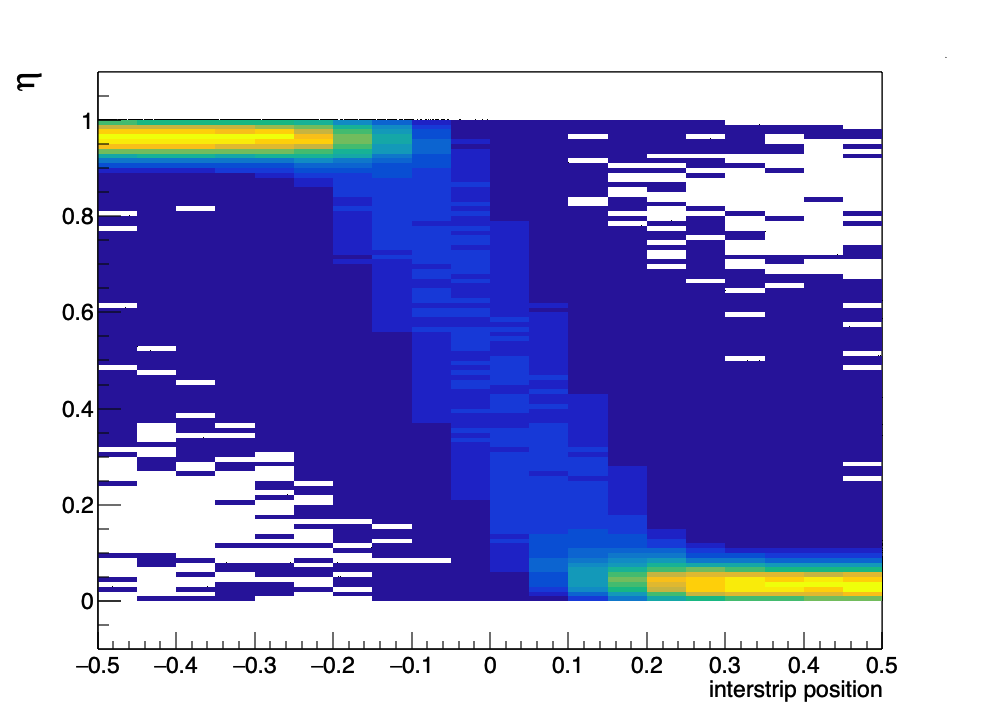
\includegraphics[width = 0.49\textwidth]{figures/eta/eta_2d_10.png} 
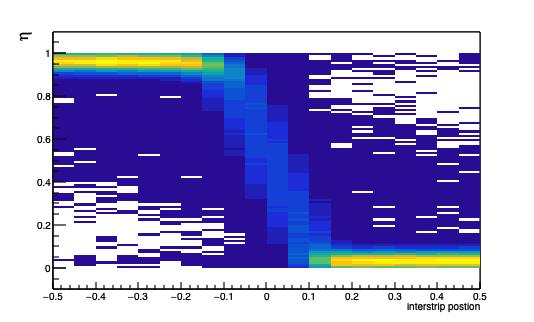
\includegraphics[width = 0.49\textwidth]{figures/eta/eta_2d_neg10.png}
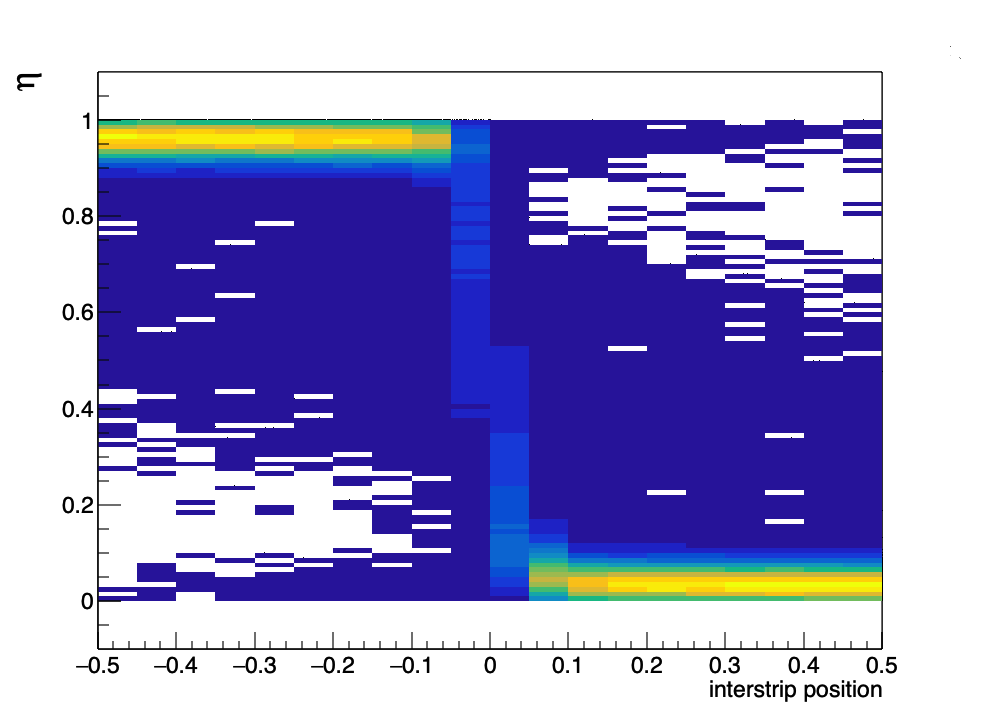
\includegraphics[width = 0.49\textwidth]{figures/eta/eta_2d_2.png} 
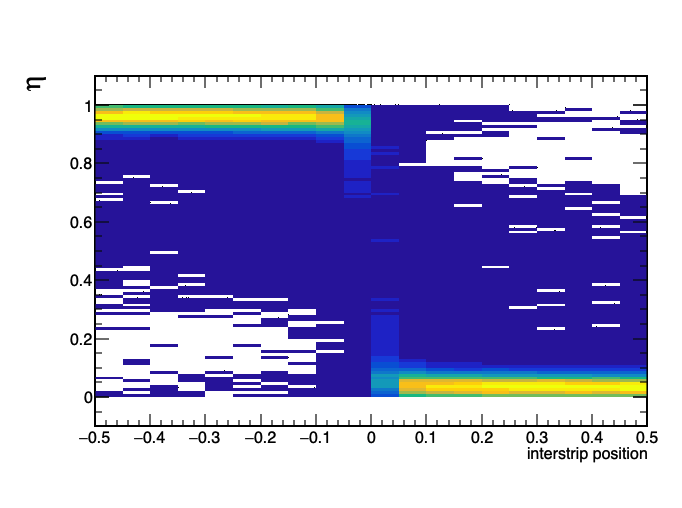
\includegraphics[width = 0.49\textwidth]{figures/eta/eta_2d_neg2.png} 
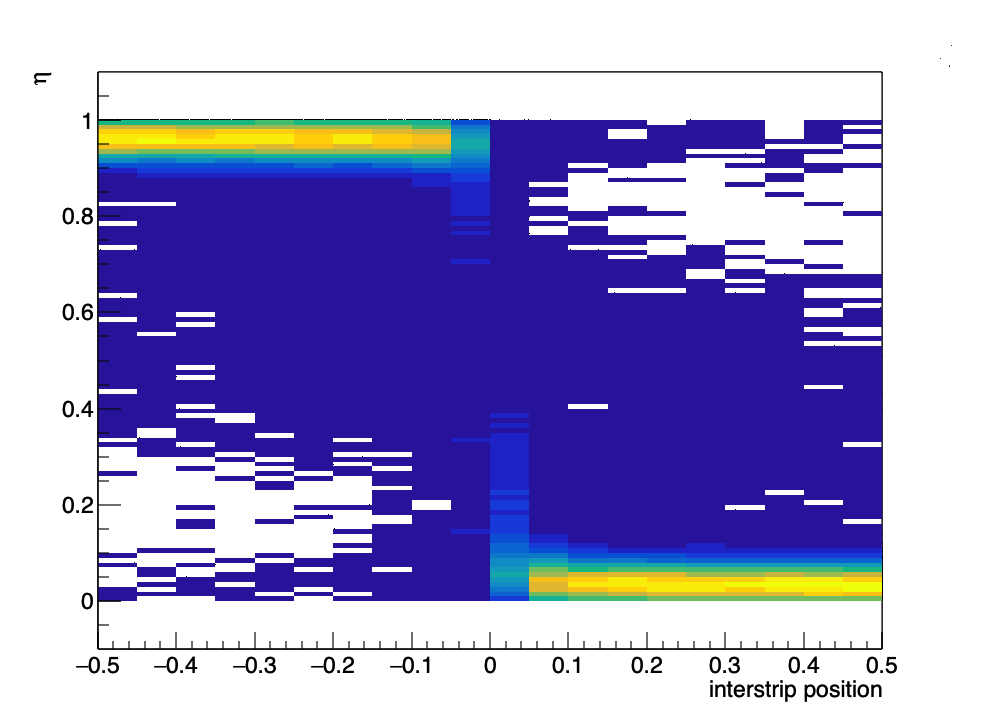
\includegraphics[width = 0.49\textwidth]{figures/eta/eta_2d_0.png} 

\caption{Distribution of a charge sharing $\eta$ versus interstrip position obtained for particles incident at a different angles. Upper row $10^{\circ}$ and $-10^{\circ}$, middle row $-2^{\circ}$ and $2^{\circ}$, bottom row $0^{\circ}$ - perpendicular to the $x$ axis.    }
\label{fig:eta_distribution_2d}
 \end{center}
 \end{figure}
 
 
 
\begin{figure}[tbph]
\begin{center}
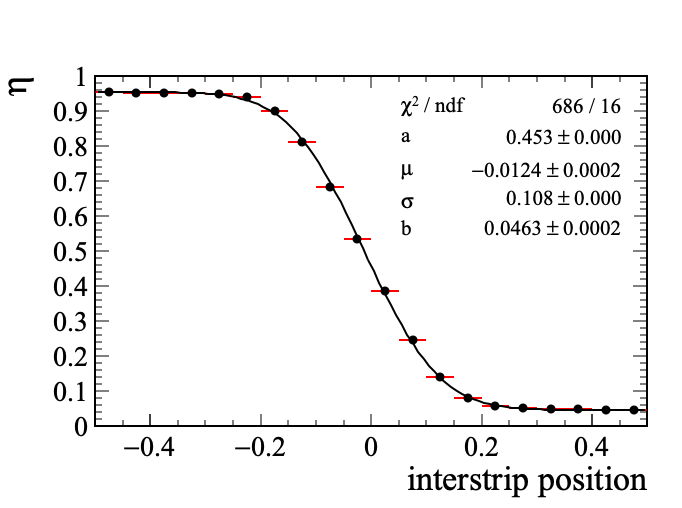
\includegraphics[width = 0.49\textwidth]{figures/eta/eta_fit_10.png} 
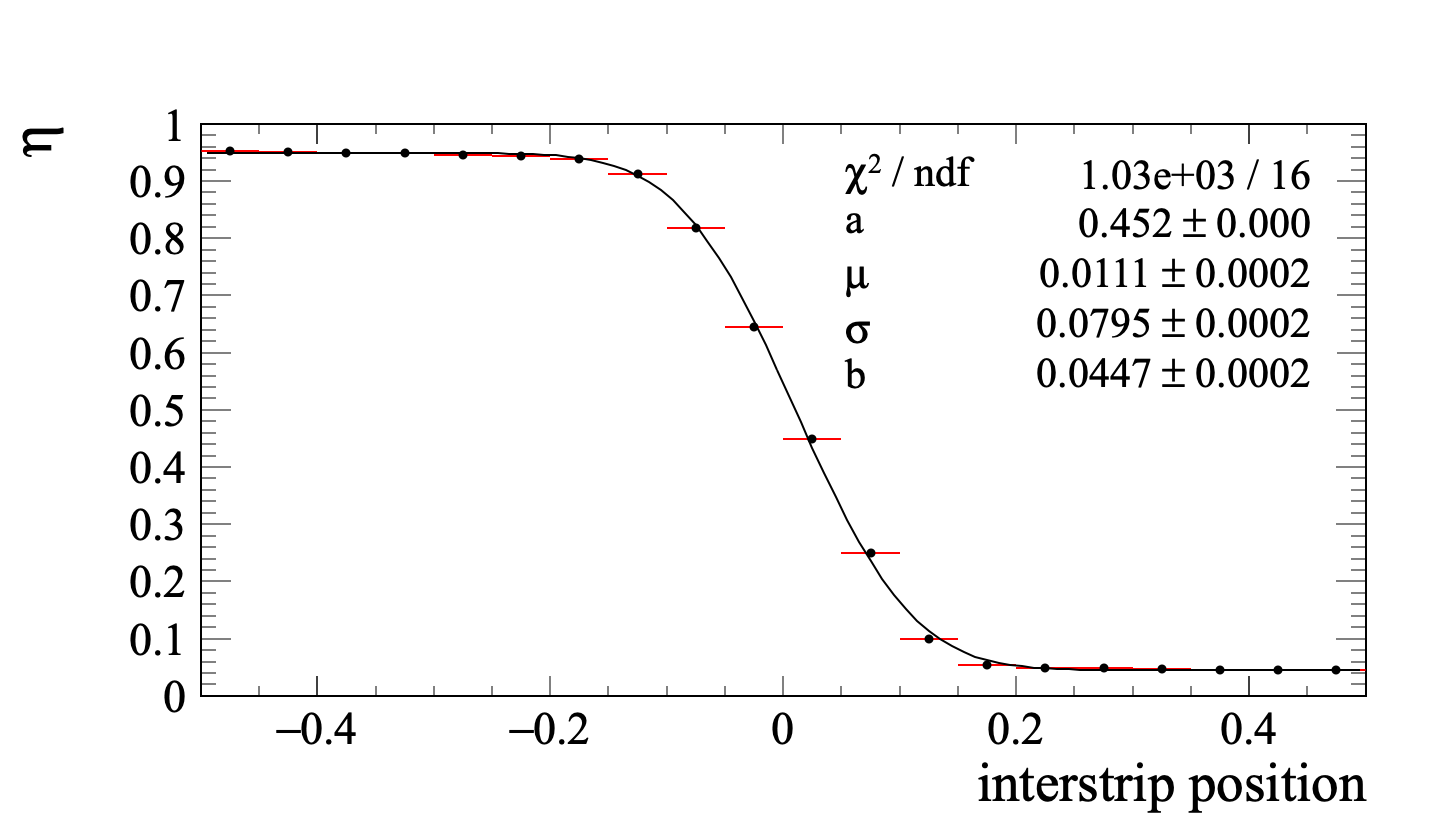
\includegraphics[width = 0.49\textwidth]{figures/eta/eta_fit_neg10.png}
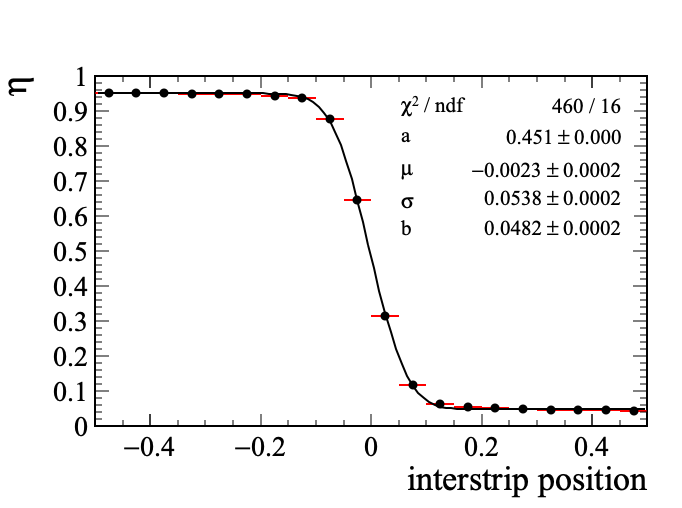
\includegraphics[width = 0.49\textwidth]{figures/eta/eta_fit_2.png} 
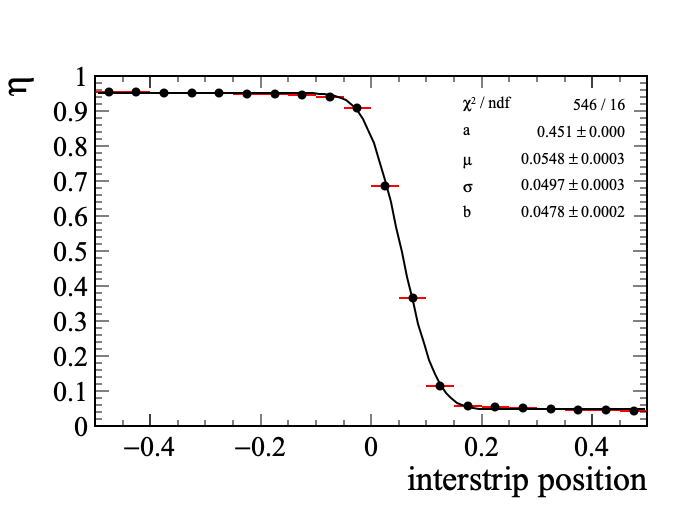
\includegraphics[width = 0.49\textwidth]{figures/eta/eta_fit_neg2.png} 
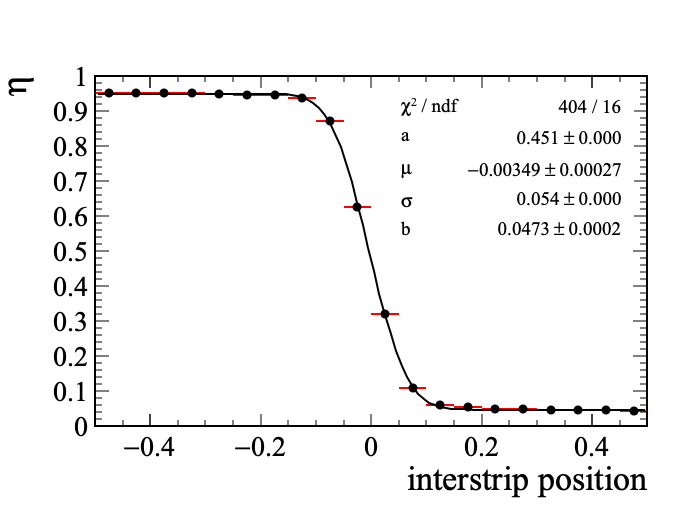
\includegraphics[width = 0.49\textwidth]{figures/eta/eta_fit_0.png} 

\caption{Charge sharing $\eta$ as a function of the cluster interstrip position obtained for different rotation angles around $y$ axis. Upper row $10^{\circ}$ and $-10^{\circ}$, middle row $-2^{\circ}$ and $2^{\circ}$, bottom row $0^{\circ}$ - perpendicular to the $x$ axis. The black solid line is a charge sharing model \ref{eq:eta_model} fitted to the data. }
\label{fig:eta_fit}
 \end{center}
 \end{figure}